\chapter{Background}
\label{cha:background}

\section{Cellular automata}\label{sec:cellular-automata-sec}

The \acf{CA} was originally proposed by Stanislaw Ulam and John Von Neumann in
the 1940s as a model of the growth of crystals and an attempt at constructing a
self-replicating system \parencite{vonneumannTheorySelfreproducingAutomata1966}.

\paragraph{Definition}
It is usually defined on a regular lattice in one or two dimension. Each of its
components is called a cell, and can be in a state $k \in \mathcal{S}$. $\mathcal{S}$ is the space of
available states for the cells, usually chosen to be $\{0, 1\}$ for binary
\acp{CA} or $\{1, \ldots, n\}$ for \acp{CA} with $n$ states.

A neighborhood function $\boldsymbol{N}$ is defined which associates each cell
with its neighbors on the lattice. In general, a \ac{CA} can be constructed on
any space $\mathcal{L}$ where such a function can be defined. The space $\mathcal{L}$ specifies an
indexing and the relation between the cells. In practice, regular finite or
infinite grids are chosen, $\mathcal{L} \subset \mathbb{Z}$ or $\mathcal{L} \subset \mathbb{Z}^{2}$. For example, the grid could
be a 1-dimensional torus with 10 cells, that is
$\mathcal{L}_{{T_{10}}} = \{1, 2, \ldots, 10 \}$. The neighborhood function has the form
\begin{equation}
  \begin{aligned}
\boldsymbol{N}_{\mathcal{L}} :\quad & \mathcal{S} \rightarrow \mathcal{S}^{s}\\
&c_{i} \mapsto [c_{j}]_{j\in \mathcal{N}_{c_{i}}}
  \end{aligned}
\end{equation}
where $\mathcal{N}_{c_{i}}$ is the neighborhood of cell $c_{i}$, $s$ is the number of
cells in the neighborhood and the returned value is a finite set of cells, the
neighbors of cell $c_{i}$. For the torus $\mathcal{L}_{T_{10}}$ above, we can define the
neighbors to be the cell itself and the two immediately adjacent cells. This
type of 1D neighborhood is illustrated on Figure \ref{fig:1d_neigh}. It
corresponds to the following neighborhood function:
\begin{equation}
  \begin{aligned}
\boldsymbol{N}_{\mathcal{L}_{T_{10}}} :\quad & \mathcal{S} \rightarrow \mathcal{S}^{3} \\
&\boldsymbol{N}_{\mathcal{L}_{T_{10}}}(c_{i}) = \begin{cases}
                      [c_{i - 1}, c_{i}, c_{i + 1}],& \text{if}\quad i \in \{2,\ldots , 9\}\\
                       [c_{10}, c_{1}, c_{2}], & \text{if} \quad i = 1 \\
                       [c_{9}, c_{10}, c_{1}], & \text{if} \quad i = 10. \\
                    \end{cases}
  \end{aligned}
  \label{eq:torus_index}
\end{equation}

On two dimensional grids, there are multiple ways to define the neighborhood.
Some common examples are the Moore neighborhood (see Figure \ref{fig:moore}) and
the Von Neumann neighborhood (see Figure \ref{fig:von_neumann}). In the rest we
omit the subscript on the neighborhood function $\boldsymbol{N}$ as we almost
always work with regular grids.

\begin{figure}[htbp]
  \centering
  \begin{subfigure}[c]{.3\linewidth}
    \centering
    
\includegraphics[width=\linewidth]{figures/1d_neigh}
    \caption{Standard 1D \ac{CA} neighborhood}
    \label{fig:1d_neigh}
  \end{subfigure}
  \begin{subfigure}[c]{.3\linewidth}
    \centering
    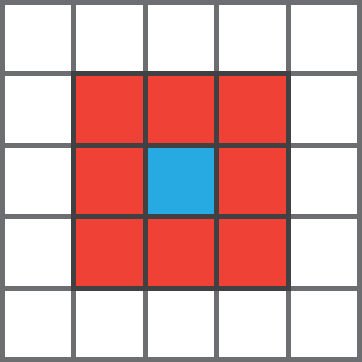
\includegraphics[width=\linewidth]{figures/moore}
    \caption{Moore neighborhood}
    \label{fig:moore}
  \end{subfigure}
  \begin{subfigure}[c]{.3\linewidth}
    \centering
    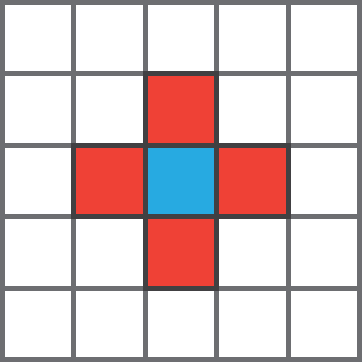
\includegraphics[width=\linewidth]{figures/von_neumann}
    \caption{Von Neumann neighborhood}
    \label{fig:von_neumann}
  \end{subfigure}

  \caption{Illustration of commonly used neighborhoods for 1D and 2D cellular automata.}
  \label{fig:neighborhoods}
\end{figure}

A \ac{CA} evolves in discrete time steps. An update rule
$\boldsymbol{\Phi}: \mathcal{S}^{s} \rightarrow \mathcal{S}$ defines the new state of a cell as a
function of its local neighborhood at the current time step. It is applied in
parallel to all the cells. For a cellular automaton in its initial state at time
step 0 --- \ie a set of cells $\left(c_{i}^{(0)}\right)_{i \in \mathcal{L}} \in \mathcal{S}^{|\mathcal{L}|}$, and a
neighborhood function $\boldsymbol{N}$, we have the following update rule
\begin{equation}
\begin{aligned}
\forall i \in \mathcal{L}, \quad c_{i}^{(t + 1)} = \boldsymbol{\Phi}\left(\boldsymbol{N}\left(c_{i}^{(t)}\right)\right)
\end{aligned}
\end{equation}

The details of an example update step on a 1 dimensional \ac{CA} is shown on
Figure \ref{fig:ca_base}. The neighborhood of the cell $c_{i}$ is itself and the
two immediately adjacent cells.

\begin{figure}[htbp]
  \centering
 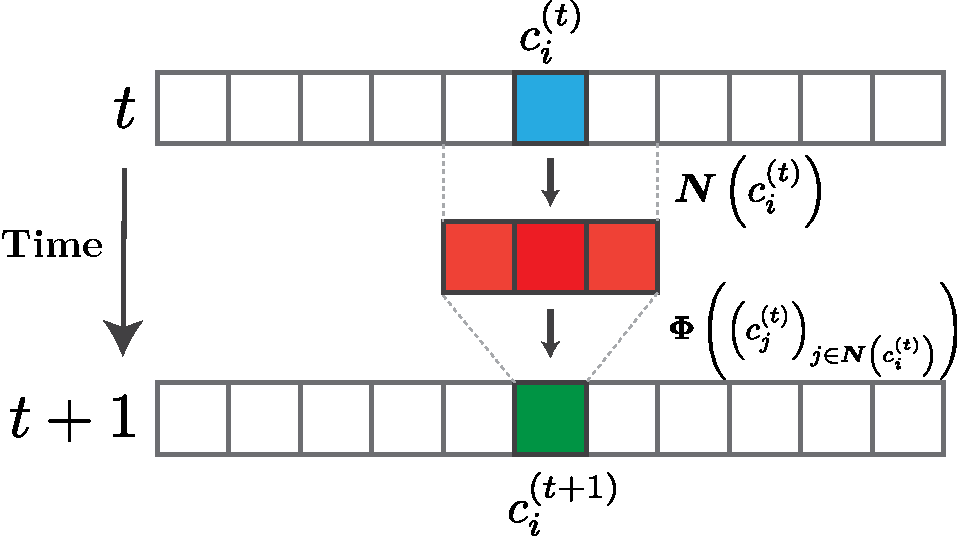
\includegraphics[width=.7\linewidth]{figures/ca_base}
  \caption{Illustration of a \acl{CA} update rule in 1 dimension. For each cell,
  we look up the neighboring cells and update its state according to the current
state of the neighbors.}
  \label{fig:ca_base}
\end{figure}

The function $\boldsymbol{\Phi}$ is often called a \emph{rule table} because it
associates an output state for each combinations of input neighbor states. These
output states can be looked up from a table containing all possible transitions
from inputs to outputs.

\paragraph{Rule representation}
A useful rule representation is obtained by listing all output state
corresponding to input configurations in a predetermined order. This results in
a list of values $[o_1, \ldots, o_{s^{|\mathcal{S}|}}]$, with $\forall i,\ o_{i} \in \mathcal{S}$, where $s$ is
the number of cells in a neighborhood, $\mathcal{S}$ is the space of available states and
$|\mathcal{S}|$ is the number of available states per cell. Using the $o_{i}$ as the
digits of a base-$|\mathcal{S}|$ number, each rule is uniquely represented by a number.
For example, as explained in more details in Section \ref{sec:elem-cell-autom},
the 256 binary rules in one dimension with neighborhood size 3 can be numbered from
0 to 255, and are referred to by their number in the literature.

\paragraph{Boundary conditions}
The grid of a \ac{CA} can be finite or infinite. In the infinite case, the grid
is assumed to be initialized to a uniform state except for a few cells set to
other states. The simulation is then run on these few cells while the rest of
the infinite grid does not have to be simulated from the start. For a finite
grid, an exhaustive simulation can be run, but there is a need to define
boundary conditions. The boundaries can be set to wrap to the other side of the
grid, forming a torus. An example of the corresponding indexing is given in
\eqref{eq:torus_index}. Other choices of boundary condition consists in adding
virtual padding cells outside of the main grid. They can be set to a fixed
state, a randomly chosen state, or mirror the cells on the inside of the grid.
Each of these choices affects the evolution and properties of the \ac{CA}, but
the importance of these boundaries decreases for very large grids.

\subsection{Classification of cellular automata}

Stephen Wolfram approached cellular automata as discrete, spatially extended
dynamical systems \parencite{wolframUniversalityComplexityCellular1984}. The
analogy is only superficial since many concepts from dynamical systems theory,
such as ``chaos'', ``attractors'' and ``sensitivity to initial conditions'' only
admit a rigourous definition in the continuous state and continuous time models.
Wolfram proposed a qualitative classification of CA behavior roughly analogous
to classifications in dynamical systems theory, with four classes defined as follows:

\begin{description}
  \item[Class 1] Initial configurations relax after a transient
        period to the same fixed configuration (e.g., all 1s).
  \item[Class 2] Initial configurations relax after a transient period to some
        fixed point or some temporally periodic cycle of configurations, but
        which one depends on the initial configuration. (\ac{CA} defined on
        finite lattices always end up having a periodic behavior because there
        is only a finite number of grid configurations. Class 2 does not refer to
        this type of periodic behavior but rather to cycles with periods much
        shorter than the total number of possible states).
  \item[Class 3] Initial configurations relax after a transient
        period to chaotic behavior. (The term “chaotic” here refers to
        apparently unpredictable space-time behavior.)
\end{description}


\subsection{Cellular automata variants}

A large number of variants of \acp{CA} have been proposed, modifying or
constraining various part of the definition above. We list some common ones
here.

\paragraph{Elementary cellular automata.\label{sec:elem-cell-autom}}
\Acp{ECA} are the 1 dimensional \acp{CA} with two states per cell and
neighborhood size 3 --- the cell and its two direct neighbors on the 1D grid.
There are 8 possible configurations of a neighborhood with 3 cells and 2 states
per cell, which corresponds to 256 possible ways to define an \ac{ECA} --- two
possible outputs for each of these 8 possible configurations, hence
$2^{8} = 256$ possible \ac{CA}. This relatively small number of rules enables
exhaustively exploring the rule space and mapping out the \ac{ECA} properties,
which would not be possible for general \acp{CA}.

\begin{figure}[htbp]
  \centering
  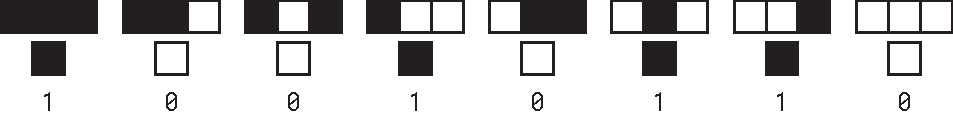
\includegraphics[width=.95\linewidth]{figures/eca_150_rule}
  \caption{Illustration of the rule of \ac{ECA} number 150.}
  \label{fig:eca_150_rule}
\end{figure}

These \acp{CA} are studied extensively, and offer an interesting combination of
trivial definition and implementation and complex and unpredictable properties.
One fundamental problem of \ac{CA} research is to classify the 256 rules into
well-defined behavior types and order them by complexity, which was attempted in
several previous works \parencite{wuenscheGlobalDynamicsCellular1992,
  gutowitzTransientsCyclesComplexity1991,
  wuenscheClassifyingCellularAutomata1999, wolframNewKindScience2002,
  zenilCompressionBasedInvestigationDynamical2010,
  hudcovaClassificationComplexSystems2020,
  hudcovaComputationalHierarchyElementary2021}.

\begin{figure}[htbp]
  \centering
\begin{subfigure}[b]{.45\linewidth}
  \centering
  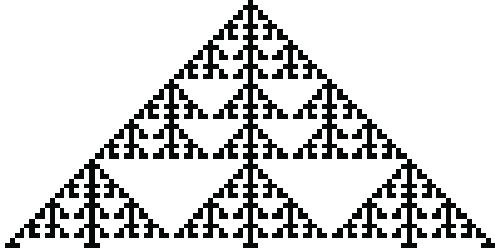
\includegraphics[width=\linewidth]{figures/eca_150_single.pdf}
  \caption{Single cell initialization}
  \label{fig:eca_150_single}
\end{subfigure}
\begin{subfigure}[b]{.45\linewidth}
  \centering
  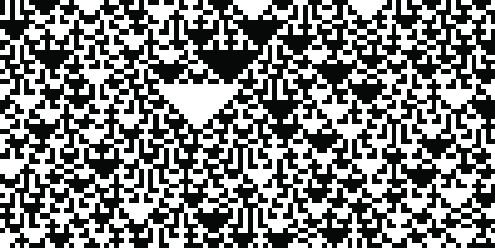
\includegraphics[width=\linewidth]{figures/eca_150_random.pdf}
  \caption{Random initialization}
  \label{fig:eca_150_random}
\end{subfigure}
\caption{Evolution of \ac{ECA} number 150 simulated on a grid of size 100 for 50
  steps. \ref{fig:eca_150_single} shows a simulation starting from a blank grid
  with only one cell set to 1. \ref{fig:eca_150_random} shows a simulation
  starting from a random initialization.}
  \label{fig:eca_150}
\end{figure}


\ac{ECA} rules are easily visualized, because there are only 8 possible
neighborhood configurations that need to be shown. For example, figure
\ref{fig:eca_150_rule} shows the transition table for \ac{ECA} rule 150. If we
assign 1 to the black state and 0 to the white state, the possible neighborhood
configurations are ordered in their binary order from right to left, with the
leftmost bit being the most significant one. This is how the rule number is
computed, using the output states (last row on figure \ref{fig:eca_150_rule}) as
a binary representation.

\paragraph{Totalistic cellular automata.}
Totalistic \ac{CA} are a subset of \ac{CA} which rules can be expressed as a
function of the sum of neighboring cell values. These \ac{CA} were introduced by
Stephen Wolfram \parencite{wolframStatisticalMechanicsCellular1983}. For
example, \ac{ECA} 150 which rule is shown on figure \ref{fig:eca_150_rule} is a
totalistic \ac{CA}. Its rule could be summarized as ``if exactly two states are
1 or all states are 0, the next state is 0, otherwise if one or three states are
1, the next state is 1''. Conway's Game of Life, presented below, is an example
of totalistic \ac{CA} in two dimensions.

\paragraph{Game of Life.\label{sec:game-life}}
The game of life is one of the most famous \ac{CA}. It was proposed by
mathematician John Conway in 1970 \parencite{gardnerMathematicalGames1970}. It
is a two dimensional binary \ac{CA}. Its two states are often called ``alive''
and ``dead''. Its rule can be summarized in three sentences as follows.
\begin{itemize}
  \item Any live cell with two or three live neighbours survives.
  \item Any dead cell with three live neighbours becomes a live cell.
  \item Other live cells and already dead cells die in the next generation.
\end{itemize}
This \ac{CA} has a particularly active community dedicated to finding
interesting patterns with particular properties such as a period length or speed
of movement through the grid. Some of these patterns have been used as memory
registers and communication channels to build a Universal Computer
\parencite{IgblanLifeUniversal}. This construction proves that the game of life
is Turing-complete. This property is thought to be also shared by other \ac{CA}
--- it is proven for at least \ac{ECA} rule 110
\parencite{cookUniversalityElementaryCellular2004}. This makes \ac{CA} models
theoretically appealing for the design of a learning algorithm because they can
simulate any algorithm.

\begin{figure}[htbp]
  \centering
  \begin{subfigure}[t]{.31\linewidth}
    \centering
    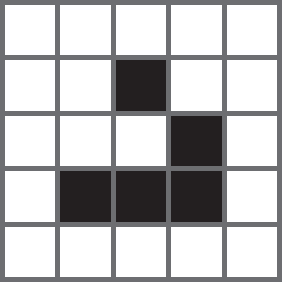
\includegraphics[width=\linewidth]{figures/glider.pdf}
    \caption{Moving oscillator (\emph{glider}).}
    \label{fig:glider}
  \end{subfigure}
  \begin{subfigure}[t]{.31\linewidth}
    \centering
    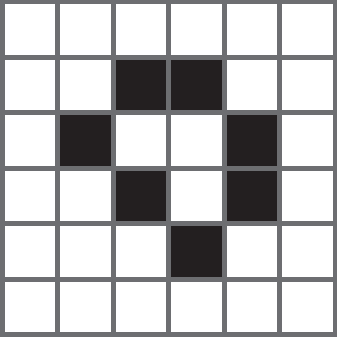
\includegraphics[width=\linewidth]{figures/still_life.pdf}
    \caption{Fixed pattern (\emph{still life}).}
    \label{fig:still_life}
  \end{subfigure}
  \begin{subfigure}[t]{.31\linewidth}
    \centering
    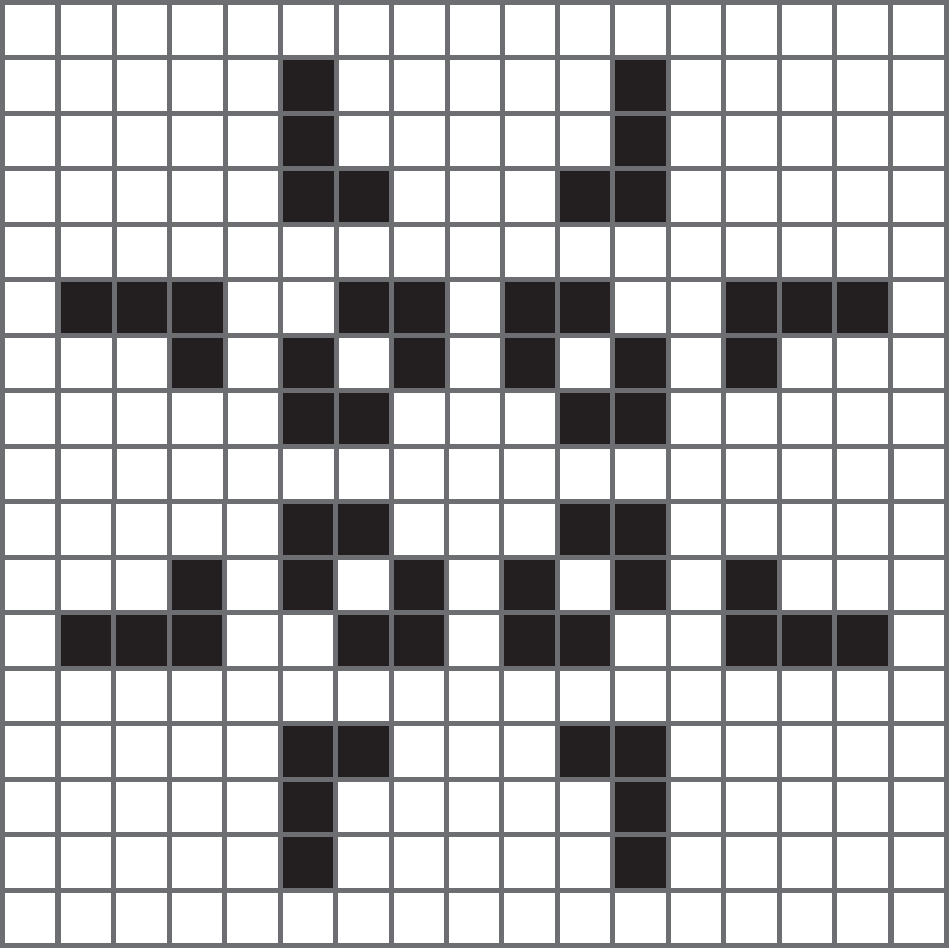
\includegraphics[width=\linewidth]{figures/pulsar.pdf}
    \caption{Period 3 oscillator (\emph{pulsar}).}
    \label{fig:pulsar}
  \end{subfigure}

  \caption{Some game of life patterns with various properties. The moving
    oscillator \ref{fig:glider} moves 1 cell along the bottom right diagonal
    every 4 steps. The fixed pattern \ref{fig:still_life} never changes except
    if it interacts with others. The oscillator \ref{fig:pulsar} loops through
    three different configurations.}
  \label{fig:gol_patterns}
\end{figure}


\paragraph{Asynchronous cellular automata}
A cellular automaton is said to be asynchronous when its cells are not all
updated in parallel at each time step. Several cell update schemes can
be chosen. Contrary to regular cellular automata, the grid has to be finite
for an update rule to exist. This is because asynchronous \ac{CA} have to define
an order of update of the cells which would not be defined on an infinite grid.
This update order can be random, follow a predefined order or be decided by a
global controller. Groups of cells can be updated simultaneously or updates can
be done cell by cell. The many effects of the asynchronous updates can be hard
to predict and make these type of \ac{CA}

Asynchronous \ac{CA} are an appealing model when using large systems for which
parallel update is prohibitively expensive. The rule could adapt itself and
preferentially update cells form active or useful parts of the \ac{CA} while
doing slower updates to the less active parts of the \ac{CA}. An asynchronous
\ac{CA} with evolutionary properties was constructed in
\parencite{nehanivEvolutionAsynchronousCellular2003}. The authors argue that
asynchronicity is a strong advantage for constructing systems that can evolve
within \acp{CA}.

\paragraph{Stochastic cellular automata}
In a stochastic cellular automaton, the update function $\boldsymbol{\Phi}$ is
stochastic. This means that the next state of all the cells of the grid is
sampled from a probability distribution that depends on the current neighborhood
configuration. We can write
\begin{equation}
\begin{aligned}
  \forall i \in \mathcal{L},\ s \in \mathcal{S} \quad p\left(c_{i}^{(t + 1)} = s \right) = \boldsymbol{\Phi} \left(\boldsymbol{N}\left(c_{i}^{(t)}\right)\right)(s).
\end{aligned}
\end{equation}
These \ac{CA} have interesting applications in physics
\parencite{vichniacSimulatingPhysicsCellular1984,
  ottaviSimulationIsingModel1989} or biology
\parencite{boasCellularPottsModel2018}.

\paragraph{Continuous}
Another family of \ac{CA} uses real-valued states, often restricted to the
range $[0, 1]$. The update function is then a real multivariate function
\begin{equation}
  \begin{aligned}
  \boldsymbol{\Phi}: [0, 1]^{s} \rightarrow [0, 1].
  \end{aligned}
  \label{eq:phi_cont}
\end{equation}

Examples of continuous \ac{CA} include Lenia
\parencite{chanLeniaBiologyArtificial2019a}, or \acp{NCA}
\parencite{mordvintsevGrowingNeuralCellular2020}.
\textcite{garzonRealComputationCellular1993} explores the condition for a
real-valued \ac{CA} to be able to compute real-valued functions.

\paragraph{Higher dimensional cellular automata}
\acp{CA} of dimension higher than 2 have been comparatively less studied for
several reasons, including the limits that arise when simulating and visualizing
systems in more than 2 dimensions on a computer screen. Another problem is with
the exploding number of possible rules in higher dimensions. The number of
neighbors per cell grows exponentially with the dimension, and the number of
possible rules has a doubly exponential rate of growth. This makes the
convenient representation of \acp{CA} rules as tables infeasible, since the size
of that table quickly exceeds the available memory of most computers. For
example, there are $2^{512} \approx 10^{154}$ possible 2D rules with 2 states and a
Moore neighborhood, which is already an incomprehensibly large number, but there
are $2^{134,217,728} \approx 10^{40,403,562}$ such rules in 3D.

Despite these limitation several works have studied higher dimensional \acp{CA},
although mostly in 3 dimensions
\parencite{tsalidesThreedimensionalCellularAutomata1989,
  sudhakaranGrowing3DArtefacts2021}. There are several examples of successful
3D \acp{CA} simulations applied to material sciences
\parencite{gandin3DCellularAutomaton1997, arataFreeformShapeModeling1999,
  panStudyFailureScale2009, dicaprio3DCellularAutomata2016}.

\paragraph{Hexagonal cellular automata}
Hexagonal cellular automata are defined on grids tiled with hexagons, where each
cell has 6 direct neighbors.

\begin{figure}[htbp]
  \centering
  \begin{subfigure}[b]{.35\linewidth}
    \centering
    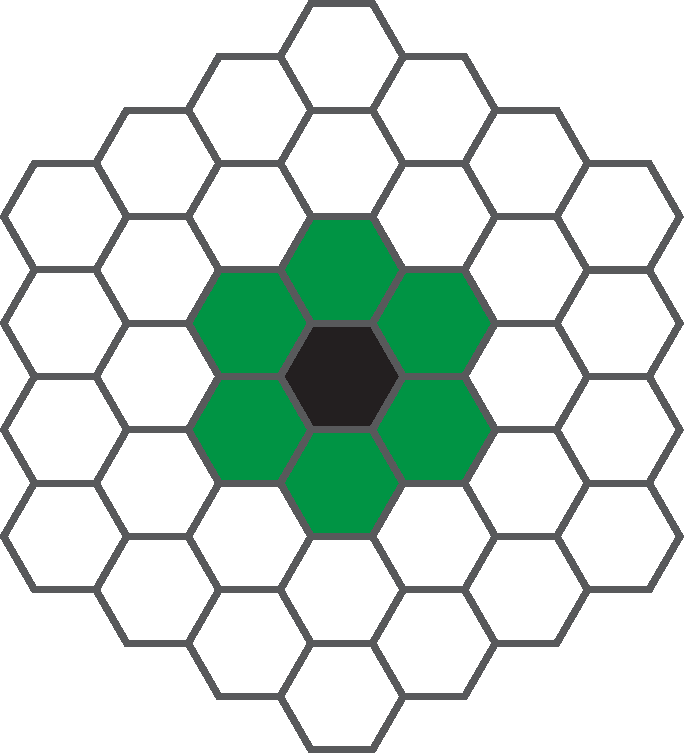
\includegraphics[width=\linewidth]{figures/hexagonal_1}
    \caption{Range 1 neighborhood}
    \label{fig:hexagonal_1}
  \end{subfigure}
  \begin{subfigure}[b]{.35\linewidth}
    \centering
    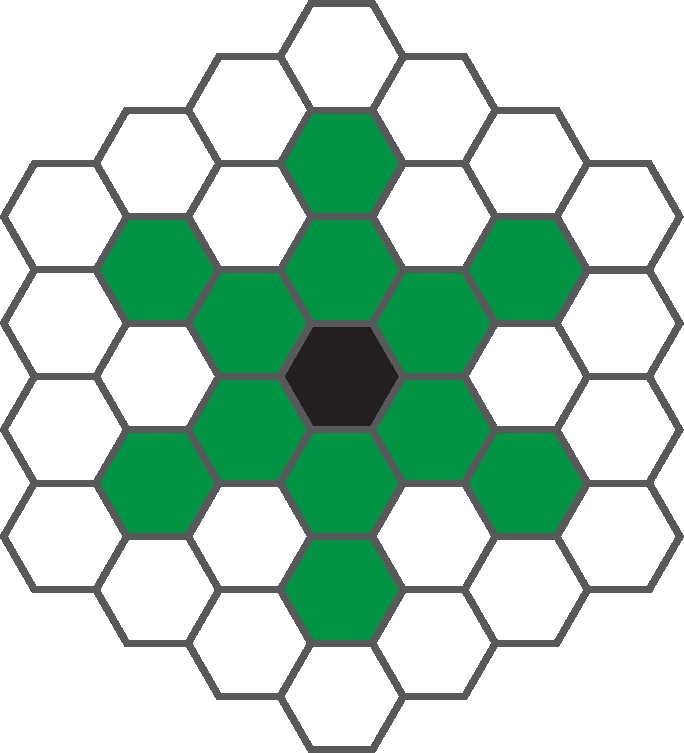
\includegraphics[width=\linewidth]{figures/hexagonal_2}
    \caption{Ray neighborhood}
    \label{fig:hexagonal_2}
  \end{subfigure}
  \caption{Example definition of neighborhood for hexagonal cellular automata.}
\label{fig:hexagonal}
\end{figure}


\subsection{Parametrizing and sampling CA rules}
As explained in \ref{sec:challenges}, one of the main challenges of working with
complex systems is the parametrization and control of the behavior of that
system. \ac{CA} are no exception, and several parametrization schemes have been
proposed, having their respective benefits and drawbacks. There are infinitely
many ways to define rules for \acp{CA}, and for each of these definition a very
large number of rules is available, making it impossible to sample a significant
portion of the rule space. A good parametrization allows scanning a wide range
of behavior of \ac{CA} by traversing the space in an interesting way.

\paragraph{Langton's lambda\label{sec:langtons-lambda}}

Christopher Langton proposed one of the first parameter that could be used to
control the behavior of \acp{CA} to some extent
\parencite{langtonStudyingArtificialLife1986, langtonComputationEdgeChaos1990}.
For a \ac{CA} with $K = |\mathcal{S}|$ states, and a state arbitrarily chosen to be
the \emph{quiescent} state (this corresponds to the ``dead'' state in the game
of life for example), if there are $n$ transitions to the quiescent state within
the rule table and $K^{s} - n$ remaining transitions that do not lead to the
quiescent state, where $s$ is the number of cells in the neighborhood, we
have

\begin{equation}
  \label{eq:langton}
  \begin{aligned}
    \lambda = \frac{K^{s} - n}{K^{n}}.
  \end{aligned}
\end{equation}

For Langton, the purpose of $\lambda$ is to search the space of \ac{CA} in an ordered
manner by varying the value of the parameter. His procedure starts with a rule
with all transitions leading to the quiescent state. The value of $\lambda$ is
increased in discrete steps up to $1 - 1 / K^{n}$ by randomly changing
transitions of the rule to lead to a different state. An illustration of the
behavior change of a \ac{CA} rule under this procedure is shown on figure
\ref{fig:langton_lambda}. Langton collects various measures of the dynamical
behavior of \ac{CA} and studies them as a function of $\lambda$. He observes a phase
transition as $\lambda$ approaches its maximal value where the \acp{CA} seem to behave
in the most complex way, with long transients and large scale propagating
structures. He calls this phase transition ``edge of chaos'' because it
corresponds to $lambda$ values just before the generated \acp{CA} become
chaotic.

\begin{figure}[htbp]
  \centering
  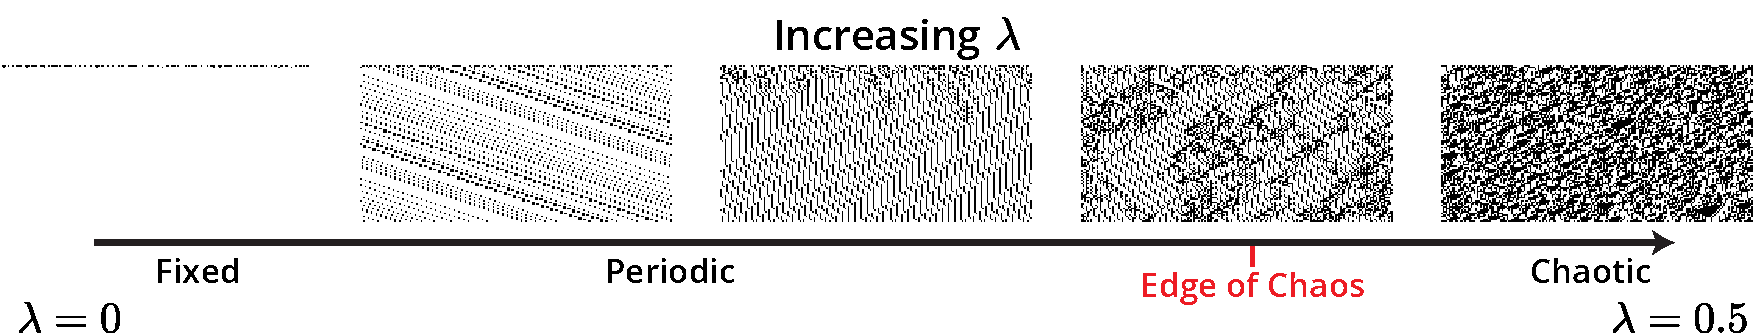
\includegraphics[width=\linewidth]{figures/langton_lambda.pdf}
  \caption{The effect of varying $\lambda$ for a 1D binary \ac{CA} rule. A \ac{CA}
    rule is progressively modified along a trajectory of increasing $\lambda$. The
    rule starts with a fixed behavior, becomes periodic and then complex when
    hitting the ``edge of chaos''. Note the localized structures that spread
    over time (down along the y axis) and interact in the fourth figure. When
    $\lambda$ increases further the rule becomes chaotic.}
  \label{fig:langton_lambda}
\end{figure}

\paragraph{Dirichlet sampling}
For an arbitrary number of states and neighborhood size, it can be challenging
to sample \ac{CA} while scanning a wide range of behavior. This is because the
size of the space of \acp{CA} rules is very large. The naive method of uniformly
sampling each transition output is not useful in large rule spaces with multiple
states, large neighborhoods or grid dimension higher than 1.

Rules with equal proportions of transitions leading to all states tend to be the
most chaotic. This is also what Langton observed when studying the $\lambda$
parameter. This is explained by the fact that sampling each transition output
uniformly is equivalent to sampling the rules from a multinomial distribution
with the number of possible states ($K$), number of possible transitions
($n = K^{K^{s}}$, with $s$ the number of cells in a neighborhood) and uniform
probabilities $p_{1}= \ldots= p_{K}$ as parameters. A random variable
$X = (X_{1}, \ldots, X_{K})$ indicates the number of times each outcome is observed.
The probability mass function of this distribution is

\begin{equation}
  \label{eq:multinomial}
  \begin{aligned}
    P(X_{1}=x_{1}, \ldots , X_{K}=x_{k}) = \frac{n!}{x_{1}!\cdots x_{K}!} p_{1}^{x_{1}}\cdots p_{K}^{x_{K}}.
  \end{aligned}
\end{equation}

This quantity gets small for large $n$ and rules with output transition skewed
towards a specific state. For example, the binary game of life rule has 372
transitions that lead to the state 0 and 140 that lead to the state 1. The
probability of sampling a rule with these transition proportions is
$8.24\mathrm{e}{-26}$, making it very unlikely to obtain such a rule with a
uniform transition sampling method.

We propose Dirichlet sampling as an alternative way to sample rules with fixed
ratio of transitions leading to output states. For a rule with $K$ states, we
sample a $K$-uple from a Dirichlet distribution of order $K$ with parameters
$(\alpha_{k})_{k\in [1, K]}$ where $\alpha_{0} = \alpha_{1} = \ldots = \alpha_{K} = \alpha < 1$. The result is a
quantile $K$-uple $(q_{1}, \ldots, q_{K})$. For $\alpha < 1$, the distribution is
concentrated around the corners of a simplex of dimension $K$.

Rules are sampled so that the number of transition to each output state matches
the quantile generated from the Dirichlet distribution. Samples will be more
likely to have a dominant quantile which can be associated with the quiescent
state in Langton's $\lambda$ calculation. The resulting sampling of cellular automata
is much better for scanning the whole space of rules and generating \ac{CA}
rules which would be unreachable with the naive sampling method, as illustrated
on figure \ref{fig:ca_rule_sampling}.

\begin{figure}[htbp]
  \centering
  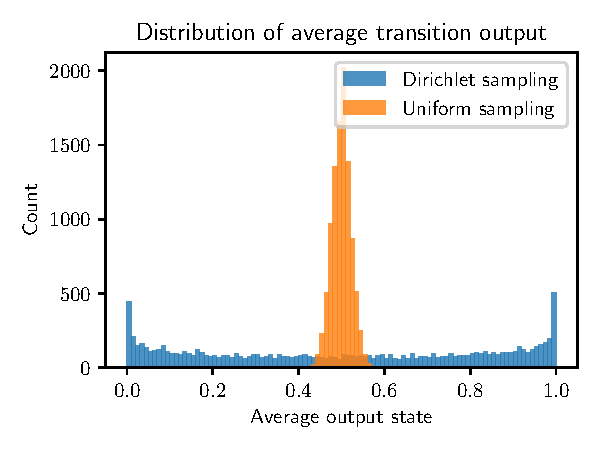
\includegraphics[width=.5\linewidth]{figures/ca_rule_sampling_hist}
  \caption{An illustration of the difference between naive uniform rule sampling
    and Dirichlet sampling on binary rules. 10000 2D binary CA rules were
    sampled with each method, the plot displays an histogram of their average
    output state. Uniform sampling leads to more rules with an average output
    state close to 0.5, meaning approximately as many transitions towards both
    states. Dirichlet sampling can control, through the choice of parameter $\alpha$,
    how much rules with more skewed transitions should be sampled which is
    visible with the spiked on the blue histogram close to 0 and 1.}
  \label{fig:ca_rule_sampling}
\end{figure}

\paragraph{Smooth sampling with the recurrent convolutional neural network
  analogy}


\section{Cellular automata and RNNs}\label{sec:cell-autom-rnns}
The purpose of this section is to show that cellular automata and recurrent
convolutional neural networks have very strong connections and to draw this
parallel as clearly as possible. We express the \ac{CA} update function as a set
of convolutional operations that can be derived from any \ac{CA} rule.

This connection yields interesting consequences both for the theoretical
properties of these models and the potential applications of cellular automata
and recurrent networks. It shows for instance that emergent properties with
increasing complexity and perhaps open-ended development are possible within the
hidden state of a recurrent neural network.

The parallel between cellular automata and a form of recurrent/convolutional
network has also been drawn by several other researchers
\parencite{wulffLearningCellularAutomaton1993,
  gilpinCellularAutomataConvolutional2018,
  mordvintsevGrowingNeuralCellular2020}.

\begin{figure}[htbp]
  \centering
  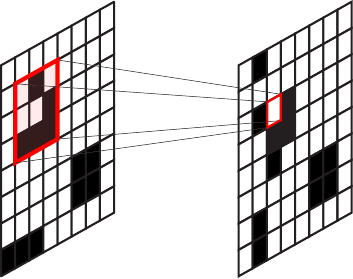
\includegraphics[width=.3\linewidth]{figures/ca_cnn}
  \caption{\label{fig:ca_cnn}The CA update rule is local and can be represented
    by a convolutional neural networks: linear local uniform transformations
    followed by the application of a non-linear function.}
\end{figure}

\subsection{RNN formalism}

\begin{figure*}[!ht]
  \centering
  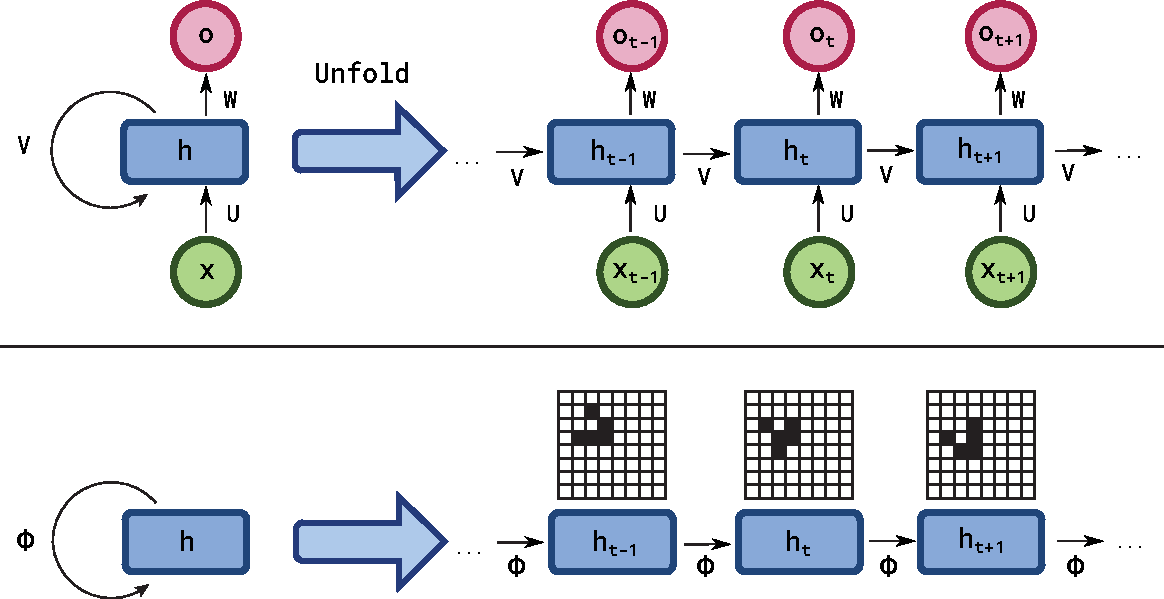
\includegraphics[width=\linewidth]{figures/rnn_and_gol.pdf}
  \caption{\label{fig:standard_rnn} Standard RNN architecture (left) and Game of
    Life seen as a RNN with no inputs and outputs (right). For the \ac{CA}, the
    ``hidden'' state $h_t$ is the current state of the grid at timestep $t$. The
    operator $\boldsymbol{\Phi}$ is the \ac{CA} update rule which is
    equivalent to a \ac{CNN} (see Section~\ref{sec:transition-rule-as}). This
    illustration is based on
    \href{https://commons.wikimedia.org/wiki/File:Recurrent_neural_network_unfold.svg}{Recurrent
      neural network unfold} by
    \href{https://commons.wikimedia.org/wiki/User:Ixnay}{fdeloche}, licensed
    under \href{https://creativecommons.org/licenses/by-sa/4.0/}{CC BY 4.0}.}
\end{figure*}


We write the definition of a cellular automaton with RNN-inspired formalism and
notations. This parallel is illustrated on Figure~\ref{fig:standard_rnn}.

The grid state at time $t$ is denoted $h_t$ and corresponds to the hidden state
in a RNN\@. In the case of classical CAs, it is a 1 or 2D vector of discrete
values, but~\parencite{mordvintsevGrowingNeuralCellular2020} and other CA
extensions use continuous values, much like the usual RNNs.

The transformation $\Phi$ operates on this hidden state only. It is equivalent
to a convolutional layer as explained below in
Section~\ref{sec:transition-rule-as}.

Inputs and outputs $(\mathbf{x}, \mathbf{o})$ are not included in the classical
definition of CAs but are an easily implementable extension as discussed in
Section~\ref{sec:adding-inputs-outp}.

\subsection{Transition rule as a set of convolutions\label{sec:transition-rule-as}}

Each cell $c_i$ from the above definition is represented as a vector of size $k$
the number of states. Cell $c_i$ is in state $s_i \in [0, \ldots, k - 1]$. A
neighborhood of size $3$ in a $1$D CA ($r=1$) is a $3 \times k$ vector
$\mathbf{u}_i = [u_{i-1}, u_{i}, u_{i+1}]$. Each $u_{ij}$ is a vector of size
$k$ with a $1$ in position $s_i$. This is illustrated in the 1D (resp.\ 2D) case
on the left (resp.\ right) of Figure~\ref{fig:cell}. For a CA with only two
states, it is redundant to have a $3\times 2$ vector, but this ``one-hot'' encoding
becomes helpful when working with more states.

\begin{figure}[htbp]
  \centering
  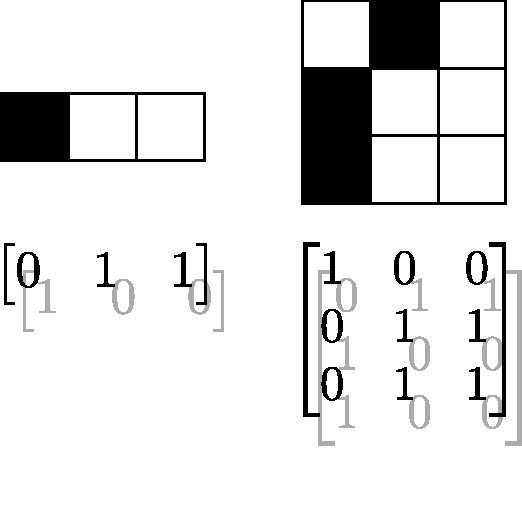
\includegraphics[width=.3\linewidth]{figures/repr}
  \caption{\label{fig:cell}Cellular automaton neighborood vector representation
    example with 2 states. A $3\times 3$ square of cells with two states can be
    represented by a $3\times 3 \times 2$ vector. Left: 1D 3-neighbors
    representation. Right: 2D $3\times3$ neighbors representation.}

\end{figure}

\begin{figure}[htbp]
  \centering
  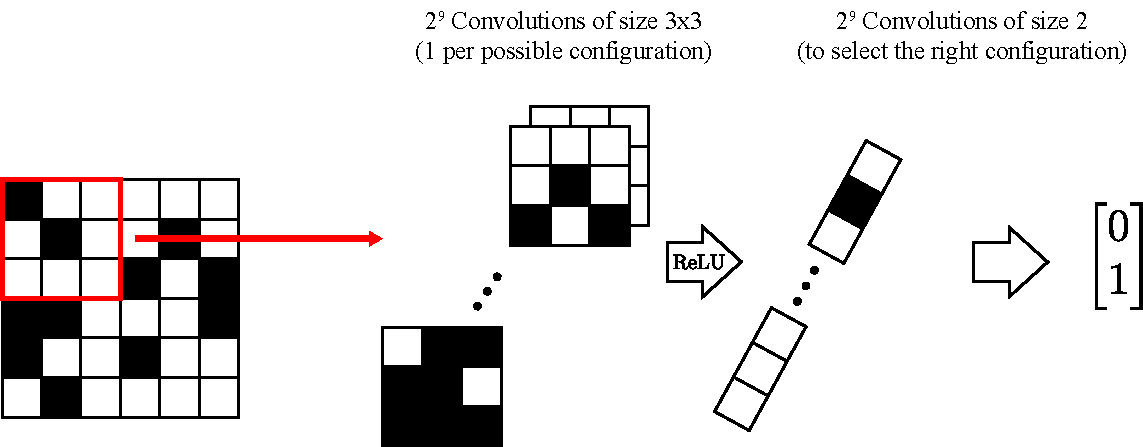
\includegraphics[width=.9\linewidth]{figures/global_schema}
  \caption{\label{fig:global_schema}How to represent any 2-states 2D CA rule
    operating on $3\times 3$ neighborhoods as a 2 layers CNN.}
\end{figure}


With this representation, on can easily express the transition rule $\Phi$ as a
simple convolutional neural network. This network would be composed of 2 layers
which are shown on Figure~\ref{fig:global_schema}:

\paragraph{The first convolutional layer}It is receptive to each possible
neighborhood configuration. This layer is composed of $k^{2r + 1}$ filters of
dimension $k\times (2r + 1)$ with only ones and zeros, that are each the same as
a possible configuration of size $(2r+1)$ of the neighborhood. The product of
each filter with an input neighborhood will be an integer between $0$ and $9$.
By applying a ReLU non-linearity with a vector of 8s as bias, we obtain the
input to the second layer, a vector of size $k^{2r + 1}$ for each cell with
plays the role of an indicator of the input configuration.

\paragraph{A second convolutional layer} It has $k^{2r + 1}$ filters of size $1$ that
are either $0$ or $1$ depending on the desired output of the transition.

\subsubsection{Recurrent convolutions in machine learning}

Recurrent convolutional networks have been used in several areas of machine
learning such as NLP or computer vision
\parencite{pinheiroRecurrentConvolutionalNeural2014,
  laiRecurrentConvolutionalNeural2015}.

\subsection{Adding inputs and outputs\label{sec:adding-inputs-outp}}

Figure~\ref{fig:standard_rnn} shows clearly where the ``missing'' inputs and
outputs could be added in Game of Life or any other CA\@. We can think of many
possible forms.

\subsubsection{Inputs}
There are many ways to add inputs to the model presented above. We divide our
proposed methods into two classes: inputs that directly modify the hidden state
during the CA evolution and inputs that augment the hidden state and affect the
rule.

\begin{description}

\item[Hidden state augmentation and rule modulation]
Inputs are usually added to the hidden state just before the application of the
non-linearity in standard RNNs.

In the case of cellular automata, it can also be done in the following ways:

\begin{figure*}[ht]
  \centering
  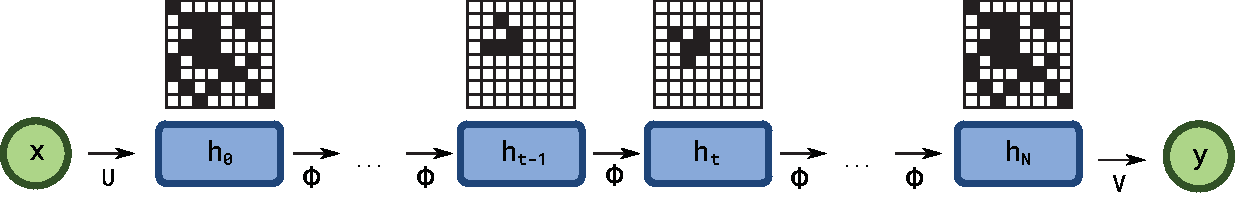
\includegraphics[width=.9\linewidth]{figures/encode_decode.pdf}
  \caption{\label{fig:encode_decode} Inputs and outputs can be directly
    encoded within the hidden state.}
\end{figure*}

\item[Vector state] A simple to add inputs to a cellular automaton is to
consider the grid as having an additional (possibly read-only) dimension. For
example, a 1D automaton would actually be represented by a vector with dimension
$N\times 2$ where the first vector of size $N$ is the grid state and the other
is the input. The update rule would be changed so as to add this new component
into account. One can see this model as using multiple CA rules at the same
time, with the input state conditioning the rule being chosen for a given update
step.

\item[Variable update rule] Inputs can also influence a CA's evolution by
changing the update rule. With this configuration, the update rule $\Phi$ is now
a function of the input $x$. We now have $\Phi_x = G(x)$, where

\[G: \mathcal{X} \rightarrow \left({\{ 1, \ldots, k \}}^{2r+1} \to \{1, \ldots, k\}\right)\]


A similar approach was used in \parencite{adamsFormalDefinitionsUnbounded2017}. It
showed that conditioning a CA update rule on another CA's evolution could enable
a higher diversity of behavior.

\item[Concatenation] Input can be concatenated to the hidden state (\eg~on
the grid boundaries) before applying the update rule, forming a sort of fixed
read-only memory space. Concatenation is illustrated in Figure~\ref{fig:concat}.
A possible disadvantage of this method is the fact that information need to
propagate through the grid if it is to be processed far from where the read-only
memory was positioned.

This approach is more computer-like, reserving some space for different
functionalities of the data.

\begin{figure}[ht]
  \centering
  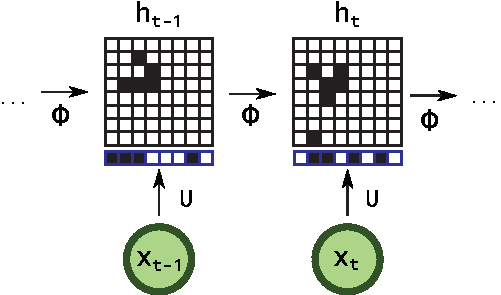
\includegraphics[width=.5\linewidth]{figures/concat.pdf}
  \caption{\label{fig:concat} Input $x_t$ is projected and concatenated to
    hidden state $h_t$, affecting the boundary conditions of the cellular
    automaton.}
\end{figure}

\item[Hidden state manipulation]

Another approach is to directly modify the hidden state to ``communicate''
information to the system. These methods are used
in~\parencite{mordvintsevGrowingNeuralCellular2020,
  randazzoSelfclassifyingMNISTDigits2020} to make interactive demos and allow
users to directly modify that hidden state. A user can interact with the
system by drawing with its mouse. This sets parts of the internal state to a
fixed cell state.

\item[Masking] Input data can serve as a mask on top of the current grid
state, forcing some cells into states that depend on the input values. If we
view the state activations in the CA as some neural pattern, this approch can
be seen as a form of \emph{neuromodulation}, which has previously been used in
machine learning \parencite{soltoggioEvolutionaryAdvantagesNeuromodulated2008,
  ishiguroNeuromodulatedControlBipedal2003,
  beaulieuLearningContinuallyLearn2020}.

A mask can be constructed from an input
vector $x$ by linearly transforming $x$ and applying an activation function
(\eg~step function). It controls which channels are activated, and where
information can flow or not. This kind of mask can be applied with element-wise
multiplication or addition but also more elaborate operations. It is illustrated
in Figure~\ref{fig:mask}.

\begin{figure}[ht]
  \centering
  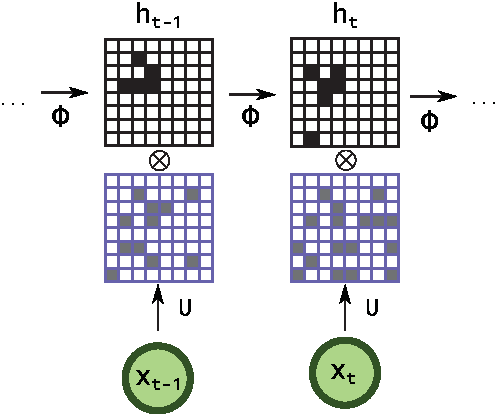
\includegraphics[width=.5\linewidth]{figures/mask.pdf}
  \caption{\label{fig:mask} Input is converted into a mask for the hidden state.
  The mask is applied through element-wise multiplication here.}
\end{figure}

\end{description}

\subsubsection{Outputs}

Similarly, inputs can be extracted from the hidden state in several different
ways. One might read outputs from the boundaries of the grid, from a
transformation of the grid using a neural network, etc. The output could also be
stored within an additional dimension of the ``extended'' grid state presented
above.

\subsubsection{Cellular automata and computations}

From a computational point of view, the hidden state can be seen as a working
tape that some kind of \emph{parallel Turing machine} (the cellular automaton)
is doing computation on. In this framework, the input is encoded as the initial
state of the tape and decoded from the last state of the tape (as illustrated on
Figure~\ref{fig:encode_decode}). The recurrent convolutional neural network
(RCNN) then plays the role of a fixed computer program. This is the setting
adopted in previous works on constructing computations with cellular automata: a
task is chosen, and one searches for rules which can execute that task on
input/output pairs~\parencite{mitchellComputationCellularAutomata2005}. Previous
successes with RNNs demonstrate that this model is powerful enough to learn
complex functions when the grid is made of continuous numbers and the
transformation is not local thanks to optimization, for instance in language
modelling.

However, this gets more interesting when we consider the input as encoding both
some data and a computer program, as it is the case with a Turing machine. We can
then expect a cellular automaton (or RNN) to not only compute the result of a particular
function, but to be equivalent to a general purpose computer capable of
computing the result of any chosen algorithm without any need for optimization.


\subsection{Consequences}

Viewing cellular automata as a recurrent convolutional neural networks  as
described above has several interesting consequences.

\subsubsection{Turing-completeness of the system}

Because we can simulate rule 110 ECA in the above system, it follows from the
Turing-completeness of this CA rule that the above system is Turing-complete.

This is a fun result, albeit not by any mean revolutionary since RNN have already
been proven to be Turing-complete~\parencite{siegelmannComputationalPowerNeural1992}.

The model is in practise relatively far from a real world CNN with a fixed
number of layers independent from one another --- compared to a variable number
of steps and shared layers for the automaton-RCNN\@.

\subsubsection{Differentiable cellular automata}

Every step of the computations involved in computing a step of a cellular
automaton represented as a RCNN is differentiable. We can therefore
theoretically couple this framework with backpropagation to make
\emph{learnable} cellular automata that can adapt their rules to minimize a
target loss function.

This is the direction taken by~\textcite{mordvintsevGrowingNeuralCellular2020}.
The authors use supervised learning on a cellular automaton and train it to get
a stable self-repairing target shape.

However, because supervised cellular automata can only do as much as they have
been trained to do, I believe it defeats the purpose of working with a model
capable of spontaneous complex emergent behavior. Open-ended complexity increase
could very unlikely be achieved through pure supervision.

\textcite{gilpinCellularAutomataConvolutional2018} takes the reverse approach, and
tries to train RCNNs to simulate a fixed CA rule, using the training process as
a way to help understand the structure of CA rule space.

\subsection{Beyond the naive rule representation}

The above representation of cellular automata rules is a one-to-one mapping.
Each automata rule has its CNN counterpart and vice versa. However, there are
more efficient ways to represent CA rules. For instance, we can make the first
layer of filters receptive both to a given configuration and its inverse
(\eg~$(1, 0, 1)$ and $(0, 1, 0)$ in a ECA) by using negative values in the
filter (use a filter $(1, -1, 1)$ instead of $(1, 0, 1)$ and $(0, 1, 0)$
separately).

For example, game of life doesn't need more than 2 convolutional filters or
parameters to be represented by a CNN because it is totalistic (a cell's new
state only depends on the number of neighbors in state 1 and its current state).


\section{Reservoir computing}



\section{Measuring complexity}

Measuring the complexity of a system is a fundamentally difficult task. Many
complex systems exhibit what Peter Grassberger calls \emph{self-generated
  complexity} \parencite{grassbergerQuantitativeTheorySelfgenerated1986}. It
means that the formulation of the problem is translationally invariant and the
observed structure arises from a spontaneous breakdown of translational
invariance. Unfortunately there is no universally accepted and formalized notion
of ``complexity'', even though most intuitively agree that it exists. No clear
observable and protocol to acquire it have been proposed that would give a
quantitative notion of complexity.

\subsection{Information based measures}


\subsubsection{Information content}
For an event $E$ with probability $P$, the information content of this event is
defined as
\begin{align*}
  I(E) := -\log(P)
\end{align*}
This measure essentially quantifies how unlikely an event is and depends on how
the probability $P$ was estimated in practice.

\subsubsection{Shannon Entropy}
It is simply the expected information content of the input.
\begin{align*}
  H(X) := \mathbb{E}[-\log(P(X))]
\end{align*}
This measure is a lower bound on the number of bits the input could be
compressed down to. In the case of a 1D ECA, the Shannon entropy could be
computed cell-wise over the time distribution of the states. Yielding an entropy
per cell score that can be averaged over a entire automaton.

This is for instance one of the measures used by Wolfram in
\parencite{wolframStatisticalMechanicsCellular1983} and by Langton in
\parencite{langtonComputationEdgeChaos1990} to study how the parameter $\lambda$ affects
the behavior of the automaton.

There are several ways to compute it when dealing with a CA, depending on what
part of the CA is considered as the main random variable. If the CA is finite,
the state at timestep $t$ can be seen as a random variable that can take one of
$2^N$ possible values (with $N$ the width of the automaton state). In that case,
the probability of a state can easily be estimated by counting its number of
occurences during evolution.

\subsubsection{Rényi Entropy}
The Rényi entropy is a generalization of Shannon entropy that gives different
weights to events of various probabilities. It is formally defined for an
$\alpha \geq 0, \alpha \neq 1$ and $X$ random variable with possible outcomes
$0, 1, ..., n$ as
\begin{align*}
  H_\alpha(X) = \frac{1}{1-\alpha} \log\left(\sum_{i=0}^np_i^\alpha\right)
\end{align*}

In the limit $\alpha \rightarrow 1$ it is equal to the Shannon entropy. $\alpha
\rightarrow \infty$ yields the Min-entropy. With $\alpha \rightarrow 0$ Rényi
entropy is the same as Max-entropy.

Rényi entropy is used in \parencite{wolframStatisticalMechanicsCellular1983} to
estimate entropy in infinite CAs.

\paragraph{Mutual information}

\subsection{Computation based measures}

\subsubsection{Kolmogorov-Chaitin complexity {\small (algorithmic complexity)}}

Introduced by Kolmogorov \parencite{kolmogorovThreeApproachesQuantitative1968} and Chaitin
\parencite{chaitinLengthProgramsComputing1969}, this complexity measure is defined for a string $s$
of characters and a universal description language (\eg a programming language)
as the length of the shortest program that can generate the string $s$. Such
number $K(s)$ is called the minimal description length of $s$.

From the invariance theorem, the difference in Kolmogorov complexity of the same
string $s$ in two different description language is bounded, although this bound
might be very large in practice.

The Kolmogorov complexity is uncomputable, and there exists strings of
arbitrarily large complexity, which makes it hopeless using this exact measure
in practice.

One rather straightforward way of approaching the Kolmogorov complexity of an
arbitrary string is to use a compression algorithm, and use the length of the
decompression program plus the length of the compressed string as an upper bound
to the Kolmogorov complexity. This is the approach adopted by Zenil in
\parencite{zenilCompressionBasedInvestigationDynamical2010} to classify the 1D ECA. This method, which
often makes use of the popular LZ algorithm can be seen as an independent
complexity measure, also closely related to the Lempel-Ziv complexity, described
in more details in~\ref{subsection:lempel-ziv}.

However, it is worth noting that in the case of a grid state generated by a
cellular automaton, the Kolmogorov complexity is easily upper bounded by a
constant value entirely defined by the transition table of the automaton, its
characteristics (size, boundary conditions, \etc), the initial state and number
of steps.

\subsubsection{Lempel-Ziv complexity}\label{subsection:lempel-ziv}
The Lempel-Ziv complexity as defined in \parencite{lempelComplexityFiniteSequences1976} is the
number of steps in the LZ algorithm, which is directly related to the number of
repeated substrings in the input string.

The main idea of this algorithm is to scan the input string while attempting to
find some repetition of previous input in the incoming data. This builds over
time a set of basic components called the exhaustive history of the string, from
which the complete string can be constructed. The number of components in that
set is the Lempel-Ziz complexity of that string.

The compressed length method of measuring complexity makes use of a compression
algorithm to reduce the size of the input. An input with regularities and
repetitive patterns will result in a small output whereas a random input will
rather be .

\subsubsection{Computational complexity}

\subsubsection{Logical Depth}

\subsubsection{Thermodynamic Depth}

\subsubsection{Sophistication}

\subsubsection{Effective Measure complexity}
